\chapter{Testy}
	Ten rozdział zawiera opis metodologii przeprowadzonych testów oraz komentuje ich wyniki. Nawet niewielkie defekty w~kodzie emulatora mogą spowodować błędne działanie programów przeznaczonych dla procesora Zilog Z80 lub wręcz uniemożliwić ich wykonanie. Dlatego dla każdej metody implementującej rozkaz procesora został opracowany co najmniej jeden test jednostkowy. Testy jednostkowe zaimplementowane przy pomocy biblioteki JUnit. Dodatkowo wykonano także testy manualne, polegające na wykonaniu programów na opracowanym emulatorze i~\emph{Z80 Simulator IDE}, a~następnie porównaniu ich wyników.
	
	\section{Testy jednostkowe}
	Testy jednostkowe to programy, które mają za zadanie weryfikować działanie określonego fragmentu testowanego oprogramowania. W omawianej aplikacji zostały użyte celem sprawdzenia czy rozkazy procesora są poprawnie emulowane.
	
	Kod testujący powstał przed napisaniem implementacji danej funkcji. Takie podejście nazywane jest \emph{Test{\dywiz}driven development}. Programista najpierw określa wymagania, jakie powinna spełniać dana metoda, a następnie pisze jej implementacje. Pozwala to na opracowanie oprogramowania o~lepszej jakości, ponieważ informatyk pisząc testy, ustala wymagania dla danego fragmentu kodu, które potem stara się spełnić\cite{tdd}.
	
	\begin{listing}[H]
		\inputminted{Java}{listings/exampleTest.java}
		\caption{Test jednostkowy instrukcji LoadAFromITest.java}
		\label{listing:LoadAFromITest}
	\end{listing}
	
	Na listingu \ref{listing:LoadAFromITest} zaprezentowano test instrukcji wczytującej zawartość rejestru \emph{I} do rejestru \emph{A} (rozkaz \emph{LD A, I}). Przedstawiony przykład pokazuje, że prosta z pozoru operacja, jaką jest pobranie wartości jednego rejestru i przeniesienie go do innego, wymaga złożonych testów.	Test sprawdza poprawność wartości umieszczonej w rejestrze docelowym, flag procesora, licznika cykli i rejestru \emph{PC} za pomocą metody \emph{assertEquals}.
	
	\section{Testy manualne}
	Testy manualne polegają na weryfikowaniu poprawności działania oprogramowania, przez człowieka, bez udziału narzędzi automatyzujących. Przeprowadza się je między innymi na poziomie interfejsu użytkownika aplikacji. Wykonano emulację przykładowych programów napisanych w~asemblerze na opracowanym oprogramowaniu i~emulatorze \emph{Z80 Simulator IDE}, a następnie porównano wyniki działania w postaci stanu rejestrów, flag i pamięci. Kody źródłowe programów zastosowanych do testów, zaczerpnięto z książki Rodney'a Zaks'a \emph{Programming the Z80}\cite{programming_the_z80}.
	
	Listing \ref{listing:findingTheLargestElementOfTable} zawiera program użyty w jednym z testów manualnych, wskazujący w tablicy liczb, element o~największej wartości. Wymaga on wprowadzenia do pamięci, począwszy od adresu \emph{30h} tablicy, której pierwszy bajt zawiera liczbę przechowywanych elementów.
	Kod programu wprowadzono zarówno do pamięci stworzonego w~ramach pracy emulatora, jak i \emph{Z80 Simulator IDE}, razem z tablicą elementów: \emph{03h}, \emph{10h}, \emph{40h}, \emph{20h}. 
	
	% przykładowy kod testujący to: http://www.z80.info/zip/programming_the_z80_3rd_edition.pdf str: 526 FINDING THE LARGEST ELEMENT OF A TABLE
	\begin{listing}[h]
		\inputminted{asm}{listings/findingTheLargestElementOfTable.asm}
		\caption{Program wskazujący największą wartość w tablicy}
		\label{listing:findingTheLargestElementOfTable}
	\end{listing}   
	  \newpage
	Zrzuty ekranów \ref{img:manualTest1Memory} i \ref{img:manualTest1MemoryIDE} prezentują pamięć obu emulatorów po wykonaniu programu. 
	Komórki o adresach \emph{50h-51h} przechowują adres, pod którym znajduje się znaleziona największa wartość w~tablicy. Oba emulatory wskazały na liczbę 40, więc poprawnie wykonały program. 
	
	\begin{figure}[h]
    		\centering
    		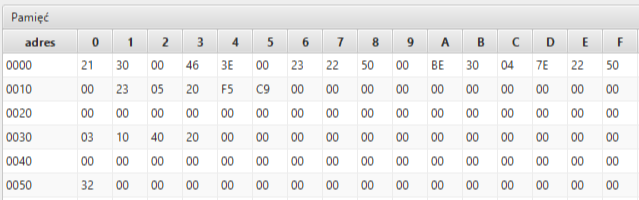
\includegraphics[width=1.0\textwidth]{manualTests/manualTest1Memory}
    		\caption{Zrzut ekranu aplikacji \emph{Z80Emu} (opracowany emulator) prezentujący pamięć procesora po wykonaniu testowego programu }
    		\label{img:manualTest1Memory}
    \end{figure}
    
    \begin{figure}[h]
    		\centering
    		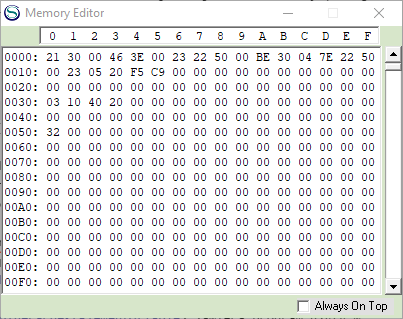
\includegraphics[width=0.6\textwidth]{manualTests/manualTest1MemoryIDE}
    		\caption{Zrzut ekranu aplikacji \emph{Z80 Simulator IDE} prezentujący pamięć procesora po wykonaniu testowego programu}
    		\label{img:manualTest1MemoryIDE}
    \end{figure}
    
    Zrzuty ekranu \ref{img:testManualnyRejestry} przedstawiają stan rejestrów, flag i liczników po wykonaniu programu. Można zauważyć, że niektóre rejestry w emulatorze \emph{Z80Emu} przyjmują wartość \emph{00h}, natomiast w \emph{ Z80 Simulator IDE} wartość \emph{FFh}. Są to rejestry, na które testowy program  nie wpływa. Nie jest to błąd. Domyślnie rejestry w Zilog-u Z80 mają wartość nieokreśloną i emulatory mogą przyjąć dowolną. Oprócz nich wszystkie wartości rejestrów, flag oraz liczników zgadzają się między obydwoma aplikacjami.
    
    \newpage
    Testowanie aplikacji było czasochłonnym i ważnym etapem przez specyfikę projektu. Emulator to program wrażliwy na błędy, i wymagane jest dokładne zweryfikowanie działania wszystkich emulowanych rozkazów procesora.
    
    \begin{figure}[h]
    		\centering
    		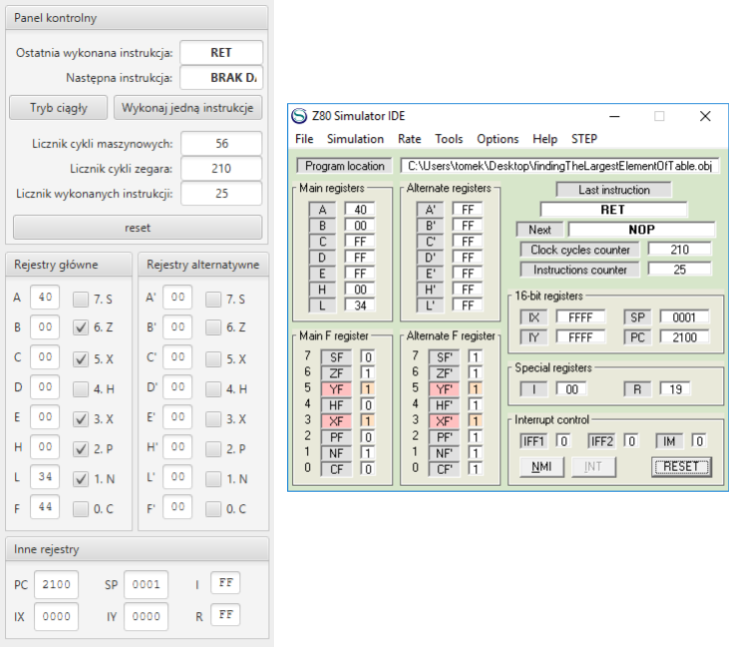
\includegraphics[width=1.0\textwidth]{manualTests/testManualnyRejestry}
    		\caption{Zrzut ekranu aplikacji \emph{Z80Emu} (po lewej) i \emph{Z80 Simulator IDE} (po prawej) prezentujący rejestry procesora po wykonaniu testowego programu}
    		\label{img:testManualnyRejestry}
    \end{figure}

    
    
    
    
    